\section{Desarrollo:} 

\begin{itemize}
	\item Crear carpetas
	\\Cree dos carpetas DATALNX DATAWIN

	\begin{center}
	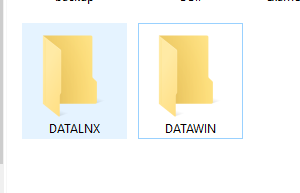
\includegraphics[width=10cm]{./Imagenes/1} 
	\end{center}

\end{itemize} 

\begin{itemize}
	\item Iniciar sesion en docker
	\\Una ves instalado docker y habilitado el Hyper-V, inicie sesion.

	\begin{center}
	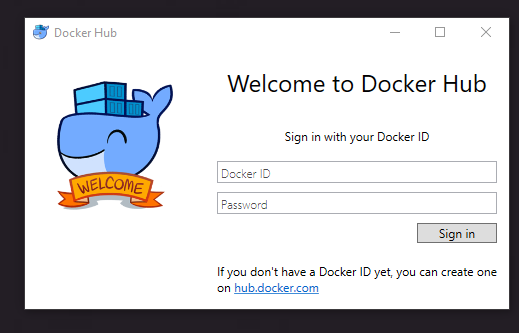
\includegraphics[width=10cm]{./Imagenes/2} 
	\end{center}

\end{itemize} 

\begin{itemize}
	\item PowerShell
	\\Habra el PowerShell con permisos de Administrador.

	\begin{center}
	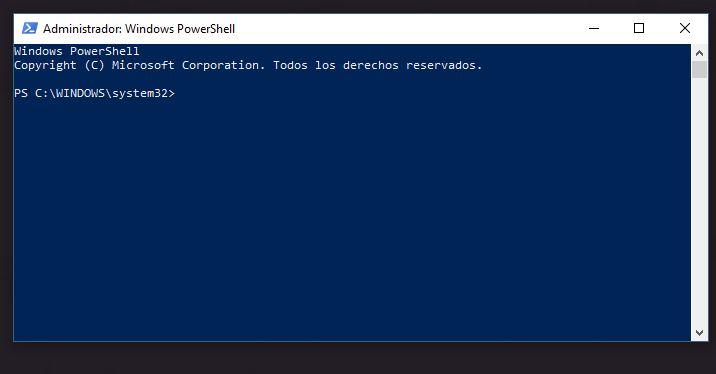
\includegraphics[width=10cm]{./Imagenes/3} 
	\end{center}

\end{itemize} 

\begin{itemize}
	\item Berifica la version de docker
	\\Use el comando "docker version"

	\begin{center}
	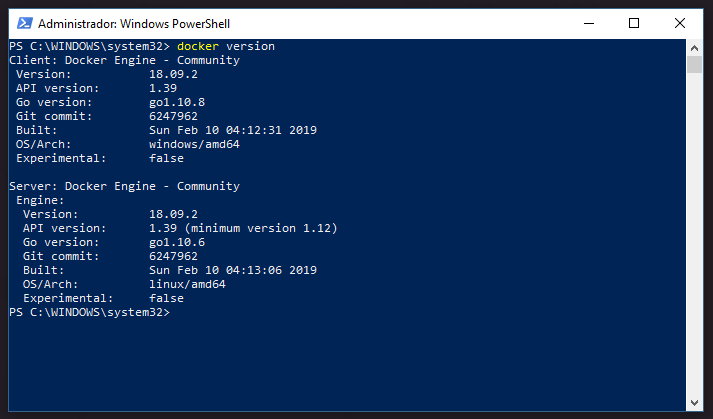
\includegraphics[width=10cm]{./Imagenes/4} 
	\end{center}

\end{itemize} 

\begin{itemize}
	\item Sql en docker
	\\Busque un contenedor con el comando "docker search mssql"

	\begin{center}
	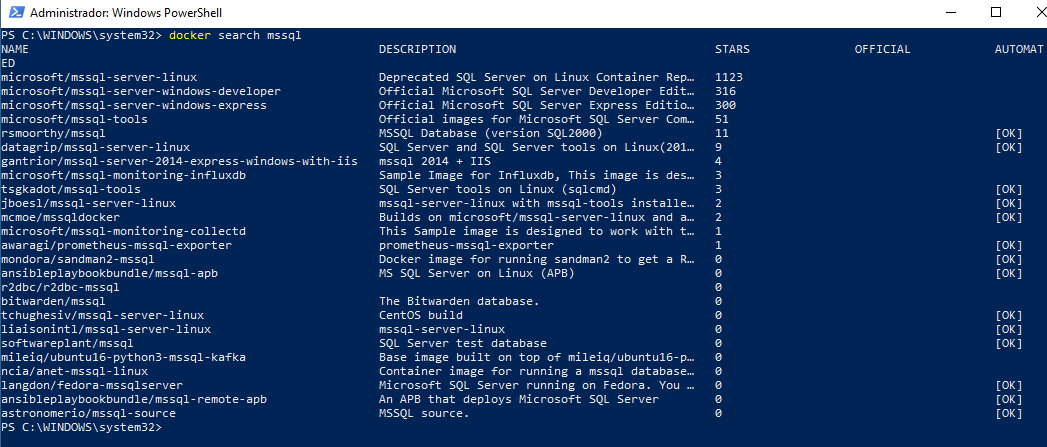
\includegraphics[width=10cm]{./Imagenes/5} 
	\end{center}

\end{itemize} 

\begin{itemize}
	\item Descargar imagen del contenedor
	\\Descargue una imagen con el comando "docker pull microsoft/mssql-server-linux"

	\begin{center}
	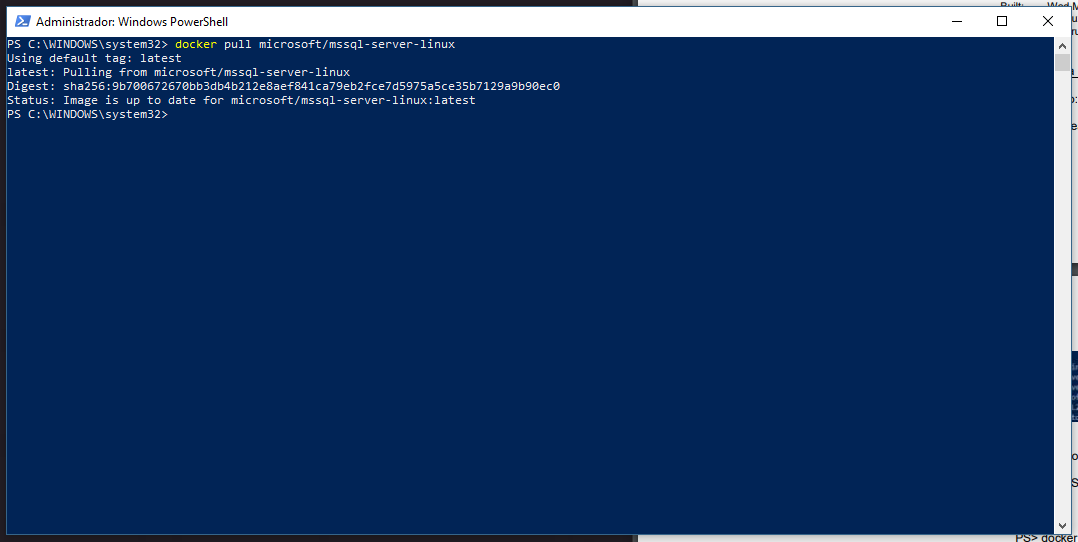
\includegraphics[width=10cm]{./Imagenes/6} 
	\end{center}

\end{itemize}

\begin{itemize}
	\item Verificar
	\\Verifique la imagen con el siguiente comando "docker images"

	\begin{center}
	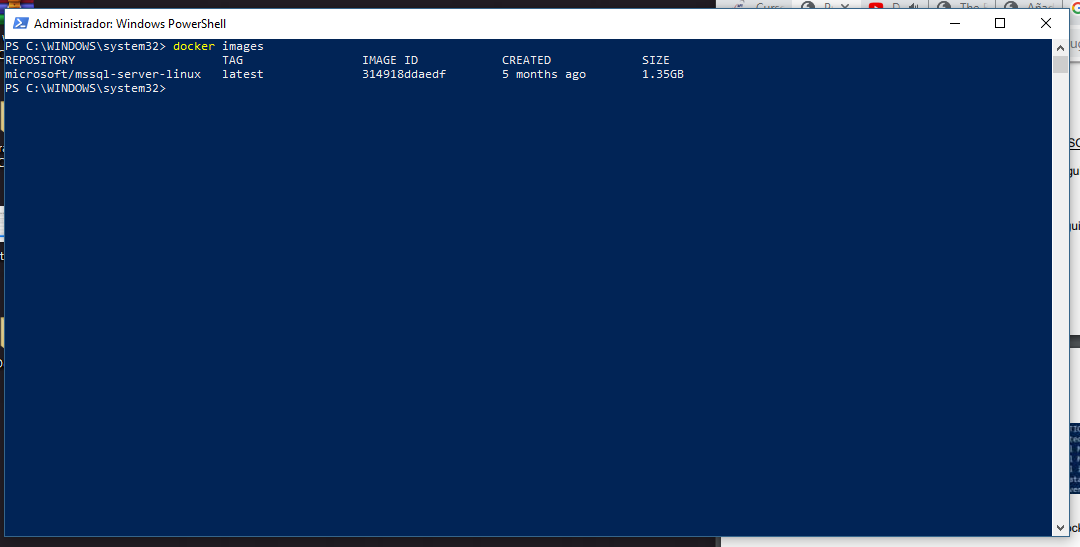
\includegraphics[width=10cm]{./Imagenes/7} 
	\end{center}

\end{itemize} 

\begin{itemize}
	\item Visualizar el ID del contenedor
	\\Usa el comando "docker run ..."

	\begin{center}
	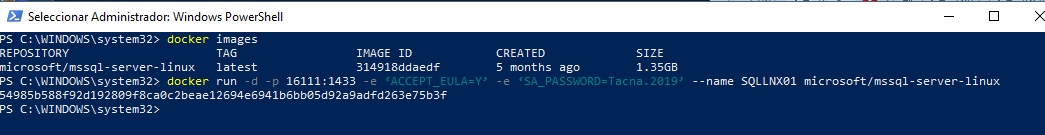
\includegraphics[width=10cm]{./Imagenes/8} 
	\end{center}

\end{itemize} 

\begin{itemize}
	\item Verificar la ejecucion del contenedor
	\\Use el comando "docker ps" para ver el estado del contenedor. Nota: Dar permisos al firewall Windows y aceptelo para realizar la conexion.

	\begin{center}
	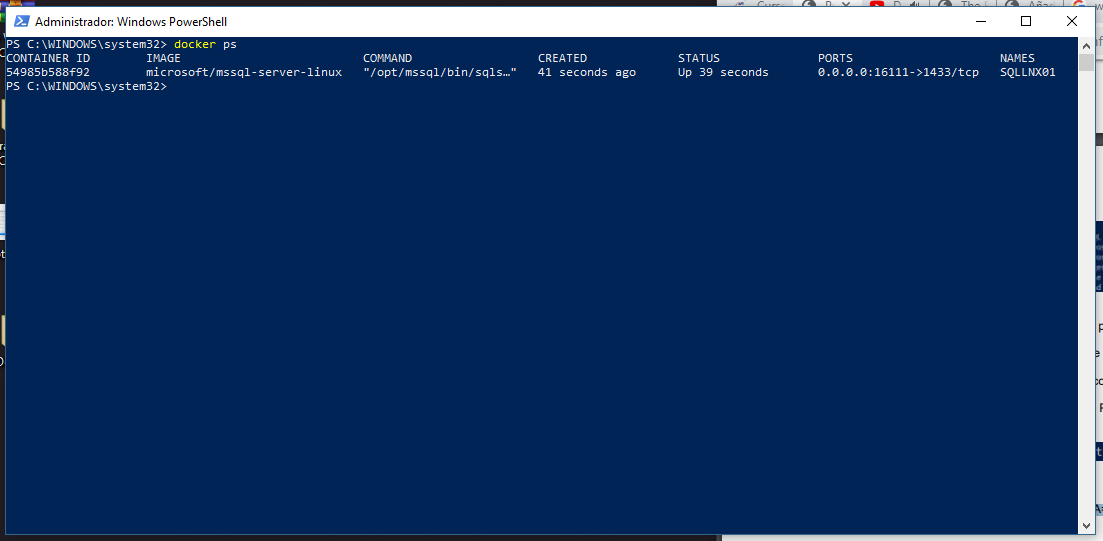
\includegraphics[width=10cm]{./Imagenes/9} 
	\end{center}

\end{itemize} 

\begin{itemize}
	\item Inicie n Microsoft SQL Server Management Studio 
	\\Conectese con los siguientes datos: \textbf{Servidor:}  (local),16111 \textbf{Autenticacion:} SQL Sever \textbf{Usuario:} sa \textbf{Clave:} Tacna.2019

	\begin{center}
	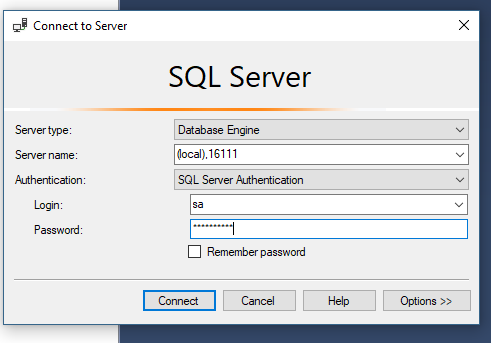
\includegraphics[width=10cm]{./Imagenes/10} 
	\end{center}

\end{itemize} 

\begin{itemize}
	\item Conexion establecida
	\\ Se ve que la conexion fue exitosa

	\begin{center}
	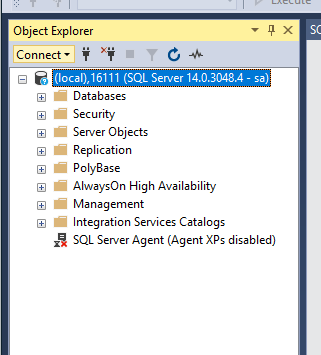
\includegraphics[width=10cm]{./Imagenes/11} 
	\end{center}

\end{itemize} 

\begin{itemize}
	\item Inicie una nueva consulta
	\\Ejecute el siguiente query SELECT @@VERSION

	\begin{center}
	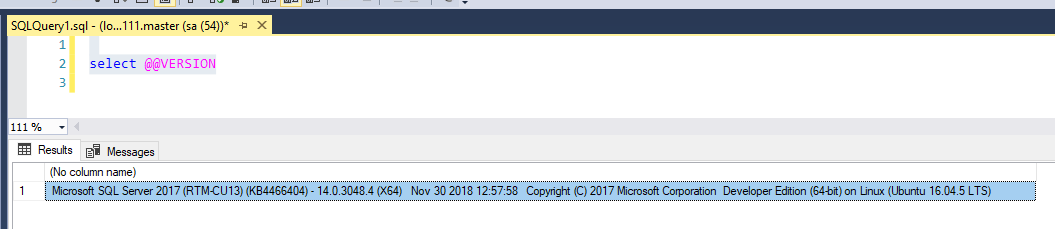
\includegraphics[width=10cm]{./Imagenes/12} 
	\end{center}

\end{itemize} 

\begin{itemize}
	\item Cierre la aplicacion y habra el PowerShell
	\\Para eliminar el contenedor se usa el comando "docker rm -f SQLLNX01", verifique el estado con el comando "docker ps"

	\begin{center}
	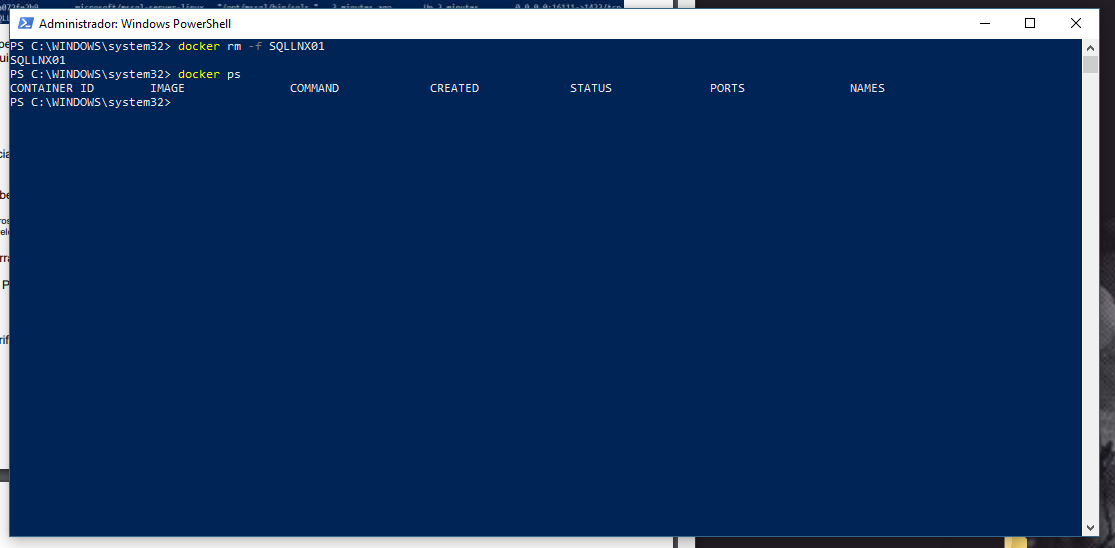
\includegraphics[width=10cm]{./Imagenes/13} 
	\end{center}

\end{itemize} 

\begin{itemize}
	\item Agregando persistencia
	\\Use el comando "docker run ..."

	\begin{center}
	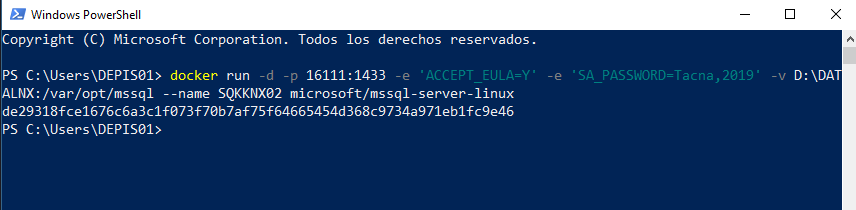
\includegraphics[width=10cm]{./Imagenes/15} 
	\end{center}

\end{itemize} 

\begin{itemize}
	\item Dar permisos
	\\Docker solicitara permisos para guardar los ficheros necesarios

	\begin{center}
	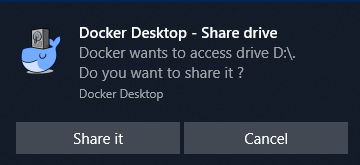
\includegraphics[width=10cm]{./Imagenes/14} 
	\end{center}

\end{itemize}  

\begin{itemize}
	\item Verifique el status
	\\Use el comando "docker ps"

	\begin{center}
	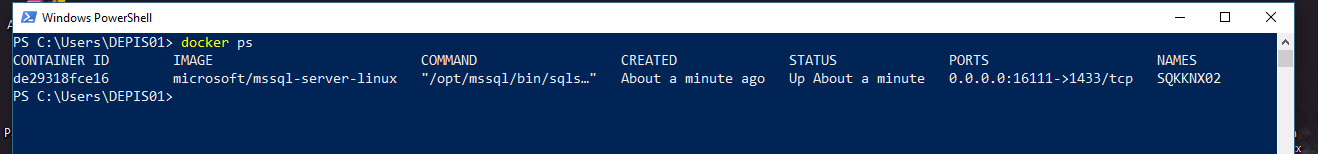
\includegraphics[width=10cm]{./Imagenes/16} 
	\end{center}

\end{itemize} 

\begin{itemize}
	\item Inicie n Microsoft SQL Server Management Studio 
	\\Conectese con los siguientes datos: \textbf{Servidor:}  (local),16111 \textbf{Autenticacion:} SQL Sever \textbf{Usuario:} sa \textbf{Clave:} Tacna.2019

	\begin{center}
	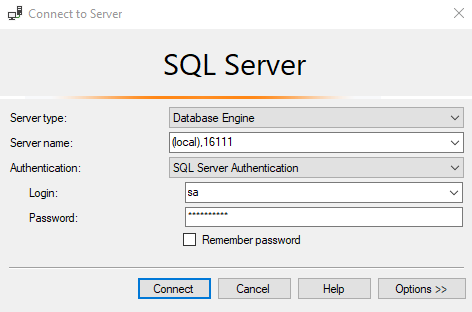
\includegraphics[width=10cm]{./Imagenes/17} 
	\end{center}

\end{itemize} 

\begin{itemize}
	\item Creado una DB
	\\Genere una base de datos a traves del siguiente query

	\begin{center}
	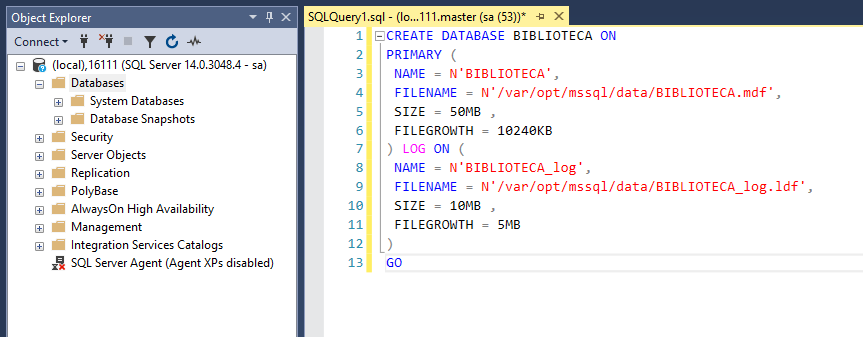
\includegraphics[width=10cm]{./Imagenes/19} 
	\end{center}

\end{itemize} 


\begin{itemize}
	\item Verificarficheros
	\\Abra la carpeta DATALINX y verifique los ficheros y carpetas

	\begin{center}
	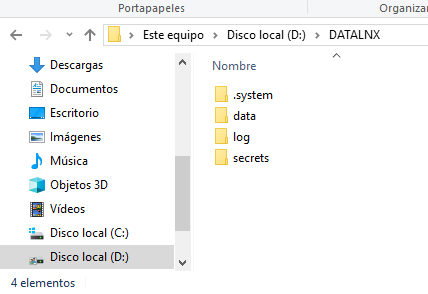
\includegraphics[width=10cm]{./Imagenes/20} 
	\end{center}

\end{itemize} 

\begin{itemize}
	\item Eliminar el contenedor
	\\Use el comando "docker rm -f SQLLNX02"

	\begin{center}
	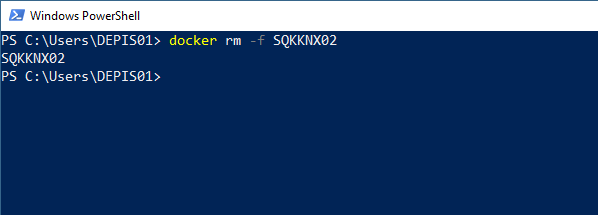
\includegraphics[width=10cm]{./Imagenes/21} 
	\end{center}

\end{itemize} 

\begin{itemize}
	\item Verificando
	\\ Use el comando "docker ps" y verifique que ya no este el contenedor

	\begin{center}
	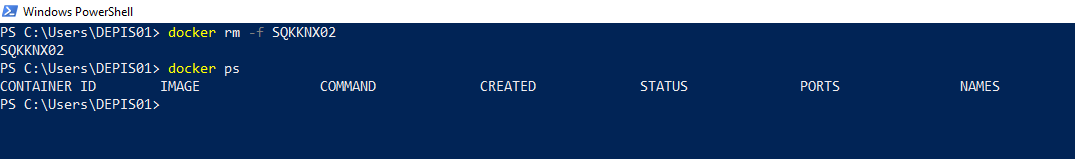
\includegraphics[width=15cm]{./Imagenes/22} 
	\end{center}

\end{itemize} 

